\chapter{Dai riconoscitori agli interpreti}

\subsubsection{Dai puri riconoscitori...}
Finora si sono considerati soltanto \textit{puri riconoscitori}, che:
\begin{itemize}
    \item accettano in ingresso una stringa di caratteri
    \item riconoscono se essa appartiene a un linguaggio
\end{itemize}

\begin{figure}[H]
    \centering
    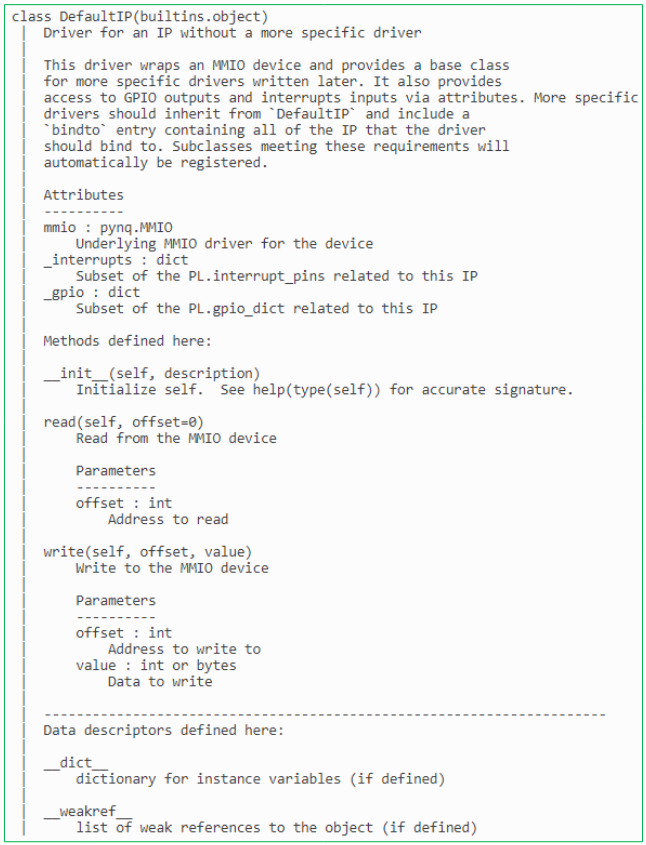
\includegraphics[width=0.8\textwidth]{/home/riccardoob/appunti/linguaggi/images/18.png}
\end{figure}

La risposta è sempre di tipo booleano, non ha importanza \textit{come} si arriva a stabilire la correttezza.

\subsubsection{...agli interpreti}
Un \textbf{interprete} è più di un puro riconoscitore, riconosce una stringa ma esegue anche azioni in base al significato (\textit{semantica}) della frase analizzata.

In questo caso diventa importante la \underline{sequenza di derivazione}.

\section{Interprete}

\subsection{Struttura}
Un interpreste è solitamente basasto su due componenti:
\begin{itemize}
    \item analizzatore lessicale, \textbf{scanner} o \textit{lexer}
    \item analizzatore sintattico-semantico, \textbf{parser}
\end{itemize}

\begin{figure}[H]
    \centering
    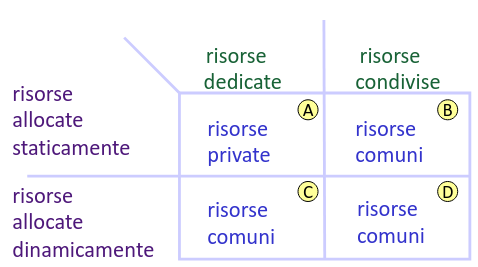
\includegraphics[width=0.8\textwidth]{/home/riccardoob/appunti/linguaggi/images/19.png}
\end{figure}

Lo scanner analizza le parti \textit{regolari} dei linguaggi, fornendo al parser singoli token già aggregati.

Il parser riceve dallo scanner i token, considerati come elementi terminali del suo linguaggio per valutare la correttezza della loro sequenza: opera sulle parti context free del linguaggio.

\subsection{Analisi lessicale}
L'analisi lessicale è la fase in cui si individuano le singole parole (token) che compongono la frase. Questa azione viene svolta raggruppando i singoli caratteri dell'input secondo \textbf{produzioni regolari} associate alle diverse possibili \textbf{categorie} lessicali.

L'analizzatore lessicale categorizza i token osservando in quale stato finale del RSF si ritrova.

\begin{figure}[H]
    \centering
    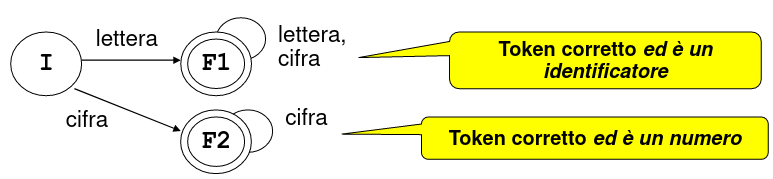
\includegraphics[width=0.8\textwidth]{/home/riccardoob/appunti/linguaggi/images/20.png}
\end{figure}

\subsection{Parole chiave}
Cablare ogni dettaglio nella struttura del RSF non è una buona strategia in quanto renderebbe estremamente complicato il riconoscitore.

\begin{figure}[H]
    \caption{Esempio riconoscimento identificatore if}
    \centering
    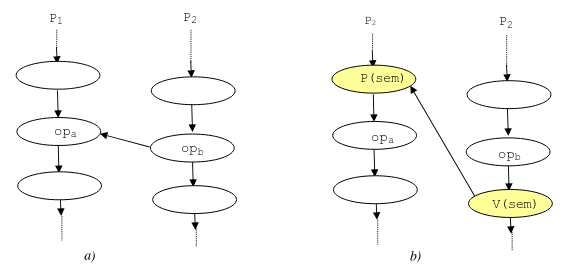
\includegraphics[width=0.7\textwidth]{/home/riccardoob/appunti/linguaggi/images/21.png}
\end{figure}

\subsection{Tabelle}
Per evitare di cablare le parole chiave, simboli etc. nella struttura del RSF, conviene agire diversamente:
\begin{itemize}
    \item categorizzare prima le parole chiave come identificatori
    \item ricategorizzare poi consultando opportune tabelle che incapsulano il dettaglio del linguaggio
    \begin{itemize}
        \item tabella \textit{parole chiave}
        \item tabella \textit{simboli}
    \end{itemize}
\end{itemize}

\subsection{Analisi sintattica top-down}
In caso di grammatiche $LL(1)$, una tecnica semplice per costruire il riconoscitore è l'analisi top-down ricorsiva discendente.

Per passare da un puro riconoscitore a un interprete occorre propagare qualcosa di più di un si o no, come ad esempio un \textbf{albero}, per una valutazione differita.

\section{Caso di studio - espressioni aritmetiche}
Si supponga di voler riconoscere espressioni aritmetiche con le quattro operazioni \textbf{+ * - /}.

\begin{figure}[H]
    \centering
    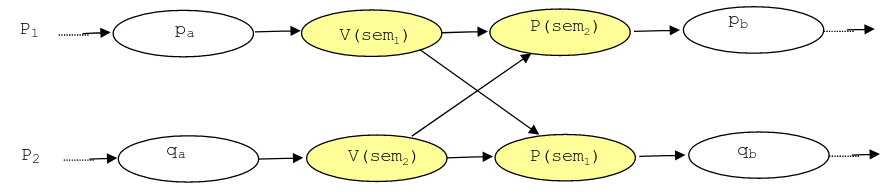
\includegraphics[width=0.8\textwidth]{/home/riccardoob/appunti/linguaggi/images/22.png}
\end{figure}

Un puro riconoscitore deve solo dire se sono corrette, ma un interprete deve anche dire:
\begin{itemize}
    \item se il dominio sono gli \textit{interi} il risultato può essere un valore int
    \item se il dominio sono i \textit{reali} il risultato può essere un valora double
    \item se l'obiettivo è la \textit{valutazione differita}, il risultato può essere un opportuno oggetto (albero)
\end{itemize}

\subsection{Analisi del dominio}

\subsubsection{Sintassi}
La notazione classica insegnata identifica i quattro operatori con i seguenti simboli: $+$, $-$, $\times$, $:$.

Sono stati sostituiti dagli informatici con $+$, $-$, $*$, $/$, spesso vengono anche usate le parentesi per esprimere una priorità associativa.

\subsubsection{Semantica}
Nel dominio aritmetico usuale:
\begin{itemize}
    \item i \textit{valori numerici} si assumono espressi in notazione \textbf{posizionale} su base dieci
    \item il significato inteso dei quattro \textit{operatori} è quello di somma, sottrazione, moltiplicazione, divisione
    \item si denotano le nozioni di priorità e associatività
    \begin{itemize}
        \item \textbf{priorità} fra operatori diversi, moltiplicativi prioritari su quelli additivi
        \item \textbf{associatività} tra operatori equiprioritari, solitamente si associa a sinistra
    \end{itemize}
\end{itemize}

\subsection{Grammatica per le espressioni}
Consideriamo il linguaggio $E(G)$ relativo alla seguente grammatica per espressioni aritmetiche;
\setlist{nosep}
\begin{itemize}[label={}]
    \item $\texttt{VN} = \{ \texttt{EXP}\}$
    \item $\texttt{VT} = \{+, *, -, :, \texttt{num}\}$
    \item $S = \texttt{EXP}$
    \item $P = \{$
    \begin{itemize}[label={}]
        \item $\texttt{EXP} := \texttt{EXP} + \texttt{EXP}$
        \item $\texttt{EXP} := \texttt{EXP} - \texttt{EXP}$
        \item $\texttt{EXP} := \texttt{EXP} * \texttt{EXP}$
        \item $\texttt{EXP} := \texttt{EXP} : \texttt{EXP}$
        \item $\texttt{EXP} := \texttt{num}$ 
    \end{itemize}
    \item $\}$
\end{itemize}
\setlist{}
É una grammatica ambigua, la semantica è informale: se \texttt{EXP} è un numero, l'espressione denota un intero e il valore dell'espression coincide con quello del numero.

\subsection{Una grammatica a "strati"}
É possibile dare una struttura \textit{gerarchica} alle espressioni, esprimendo così intrinsicamente priorità e associatività degli operatori.
\setlist{nosep}
\begin{itemize}[label={}]
    \item $\texttt{VN} = \{ \texttt{EXP}, \texttt{TERM}, \texttt{FACTOR}\}$
    \item $\texttt{VT} = \{+, *, -, :, (, ), \texttt{num}\}$
    \item $S = \texttt{EXP}$
    \item $P = \{$
    \begin{itemize}[label={}]
        \item $\texttt{EXP} := \texttt{TERM}$
        \item $\texttt{EXP} := \texttt{EXP} + \texttt{TERM}$
        \item $\texttt{EXP} := \texttt{EXP} - \texttt{TERM}$
        \item $\texttt{TERM} := \texttt{FACTOR}$
        \item $\texttt{TERM} := \texttt{TERM} * \texttt{FACTOR}$
        \item $\texttt{TERM} := \texttt{TERM} : \texttt{FACTOR}$
        \item $\texttt{FACTOR} := \texttt{num}$
        \item $\texttt{FACTOR} := ( \texttt{EXP})$
    \end{itemize}
    \item $\}$
\end{itemize}
\setlist{}
Ogni strato considera \textit{terminali} gli elementi linguistici definiti in altri strati:
\begin{itemize}
    \item \texttt{EXP} considera terminali $+$, $-$ e \texttt{TERM}
    \item \texttt{TERM} considera terminali $*$, $:$ e \texttt{FACTOR}
    \item \texttt{FACTOR} considera terminali \texttt{num}, $($, $)$, e \texttt{EXP}
\end{itemize}

Le \textit{somme} e \textit{sottrazioni} aggregano i \underline{termini}, le \textit{moltiplicazioni} e \textit{divisioni} aggregano i \underline{fattori} e i \textit{fattori} sono entità \underline{atomiche}.

\begin{figure}[H]
    \caption{Priorità operatori}
    \centering
    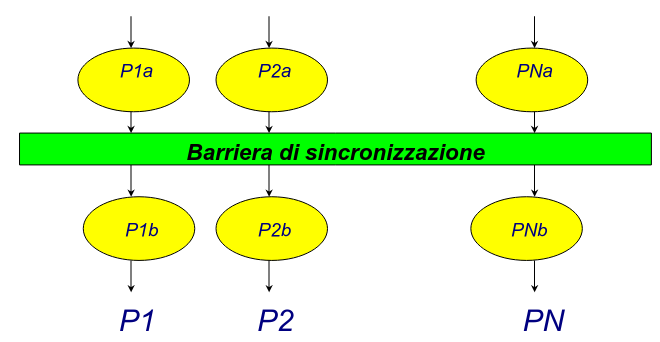
\includegraphics[width=0.8\textwidth]{/home/riccardoob/appunti/linguaggi/images/23.png}
\end{figure}

\subsubsection{Esempi}

\begin{multicols}{2}
    Frase:\\
    \noindent
    $(0111 + 0011) * 0010$\\
    Albero di derivazione
    \begin{multicolfigure}
        \centering
        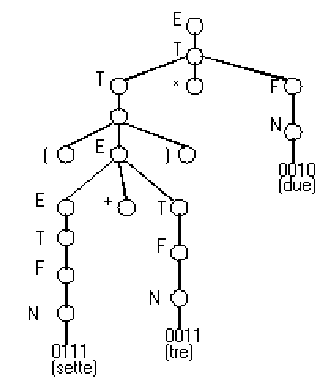
\includegraphics[width=0.7\textwidth]{/home/riccardoob/appunti/linguaggi/images/24.png}
    \end{multicolfigure}
    \columnbreak
    Frase:\\
    \noindent
    $0111 + 0011 + 0010$\\
    Albero di derivazione
    \begin{multicolfigure}
        \centering
        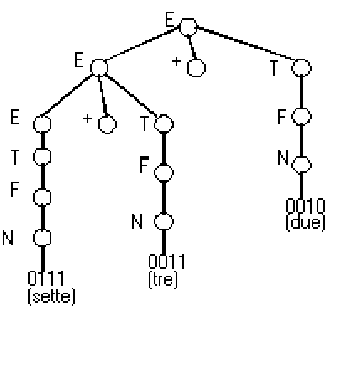
\includegraphics[width=0.7\textwidth]{/home/riccardoob/appunti/linguaggi/images/25.png}
    \end{multicolfigure}
\end{multicols}

La grammatica individuata è \textit{ricorsiva a sinistra} per esprimere la corretta associatività, tuttavia è incompatibile con l'analisi ricorsiva discendente, utile per la costruzione del parser.

\subsection{Variante 1 - Associativa a destra}
Se si riscrivono le regole in forma ricorsiva a destra, ovvero invertendo \texttt{TERM} e \texttt{EXP} e \texttt{FACTOR} e \texttt{TERM}, si otterrebbe una associatività inversa rispetto a quella usuale.

Ad esempio l'espressione $7 - 3 - 2$ verrebbe derivata come $7 - ( 3 - 2 )$ anziché come $( 7 - 3 ) - 2$.

\setlist{nosep}
\begin{itemize}[label={}]
    \item $\texttt{VN} = \{ \texttt{EXP}, \texttt{TERM}, \texttt{FACTOR}\}$
    \item $\texttt{VT} = \{+, *, -, :, (, ), \texttt{num}\}$
    \item $P = \{$
    \begin{itemize}[label={}]
        \item $\texttt{EXP} := \texttt{TERM}$
        \item $\texttt{EXP} := \texttt{TERM} + \texttt{EXP}$
        \item $\texttt{EXP} := \texttt{TERM} - \texttt{EXP}$
        \item $\texttt{TERM} := \texttt{FACTOR}$
        \item $\texttt{TERM} := \texttt{FACTOR} * \texttt{TERM}$
        \item $\texttt{TERM} := \texttt{FACTOR} : \texttt{TERM}$
        \item $\texttt{FACTOR} := \texttt{num}$
        \item $\texttt{FACTOR} := ( \texttt{EXP})$
    \end{itemize}
    \item $\}$
\end{itemize}
\setlist{}


\subsection{Variante 2 - Non associativa}
Si potrebbe anche fare a meno dell'associatività, mantenendo però lo stesso ordine di priorità. Queste regole non usano ricorsione, ne destra ne sinistra, risolvendo il problema \textit{obbligando a usare le parentesi}.

\setlist{nosep}
\begin{itemize}[label={}]
    \item $\texttt{VN} = \{ \texttt{EXP}, \texttt{TERM}, \texttt{FACTOR}\}$
    \item $\texttt{VT} = \{+, *, -, :, (, ), \texttt{num}\}$
    \item $P = \{$
    \begin{itemize}[label={}]
        \item $\texttt{EXP} := \texttt{TERM}$
        \item $\texttt{EXP} := \texttt{TERM} + \texttt{TERM}$
        \item $\texttt{EXP} := \texttt{TERM} - \texttt{TERM}$
        \item $\texttt{TERM} := \texttt{FACTOR}$
        \item $\texttt{TERM} := \texttt{FACTOR} * \texttt{FACTOR}$
        \item $\texttt{TERM} := \texttt{FACTOR} : \texttt{FACTOR}$
        \item $\texttt{FACTOR} := \texttt{num}$
        \item $\texttt{FACTOR} := ( \texttt{EXP})$
    \end{itemize}
    \item $\}$
\end{itemize}
\setlist{}






























